\section{Deinstall packages}
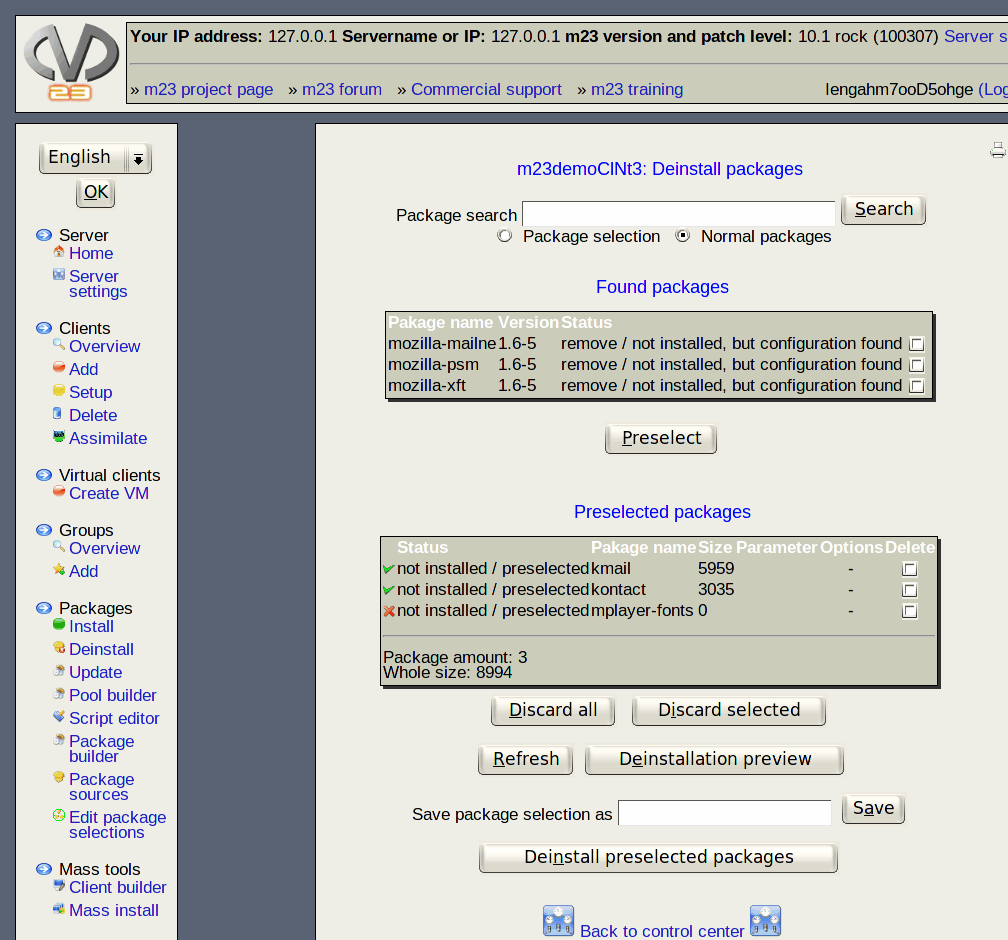
\includegraphics[scale=0.4]{/mdk/doc/manual/screenshots/en/deinstall_packages.png} \\
In this dialog you can remove packages from clients.\\
\subsection{Hint}
m23 differentiates between three kinds of packages:\\
\begin{itemize}
\item \textbf{Package selection:} Are a selection of different software packages. You can make selections like \textit{"office selection"} or \textit{"graphic workstation selection"}. So you don't have to select each single software package but you can use the package selection.\\
\item \textbf{Normal packages:} Are the normal software packages. They are mostly single applications.\\
\item \textbf{Special packages (for skilled users only):} Are packages for special tasks like formatting, setting of network options etc. Special packages should only be used by skilful users.\\
\end{itemize}
\subsection{Deinstallation of packages:}
\begin{enumerate}
\item  Select \textit{"Package selection"} or \textit{"Normal packages"}.\\
\item  Enter your search key at \textit{"Package search"}. If you leave the field blank all packages of the client.\\
\item  At \textit{"Found packages"} you can see all packages matching your search criteria.\\
\item  Check the checkbox beside all the packages you want to remove.\\
\item  Preselect your chosen packages by clicking on \textit{"Preselect"}.\\
\item  Repeat step 1-5 if required.\\
\end{enumerate}
Complete the deinstallation by clicking on \textit{"Deinstall preselected packages"}.\\
Now you have preselected packages for deinstallation. A green check mark shows that the package will be installed on the client and a red cross that the package will be removed. You can remove packages from the deinstallation list by checking the packages and clicking on \textit{"Discard selected"} or remove all by a click on \textit{"Discard all"}.\\
\subsection{Deinstallation preview}
Before you start the real deinstallation, you can test what will happen during deinstallation. You can check, which additional packages will be removed or if there will be problems. Simply click on the \textit{"Deinstallation preview"} button. After a short time you will see the previewed deinstallation protocol.\\
A deinstallation preview works for a single client only.\\
\subsection{Hint for package selections}
If you select a package selection, you can choose the action for the packages. You have the possibility to install or deinstall the packages on or from the client. Or you can keep the stored action. This makes it possible to store installation and deinstallation jobs in the same package selection. Simply select the desired action from the selection list.\\
\subsection{Hint}
If you want to save your package selection, enter a name for the selection at \textit{"Save package selection as"} and click the \textit{"Save"} button. Afterwards, you can use your selection as a \textit{"Package selection"}.\\
